% Free-floating cylinder: drained boundary and isostatic (3-2-1) support of the gel.
% Build: pdflatex hill_cylinder_free_bcs.tex && pdftocairo -svg hill_cylinder_free_bcs.pdf hill_cylinder_free_bcs.svg
\documentclass[tikz,border=4pt]{standalone}
\usetikzlibrary{arrows.meta,calc}
\tikzset{
	edge/.style={thick},
	hidden/.style={thin,dashed,gray},
	drained/.style={fill=cyan!10},
	ax/.style={-{Latex[length=2mm]}},
	support/.style={fill=red!70!black},
	block/.style={-{Latex[length=1.6mm]},red!70!black,thick},
}
\begin{document}
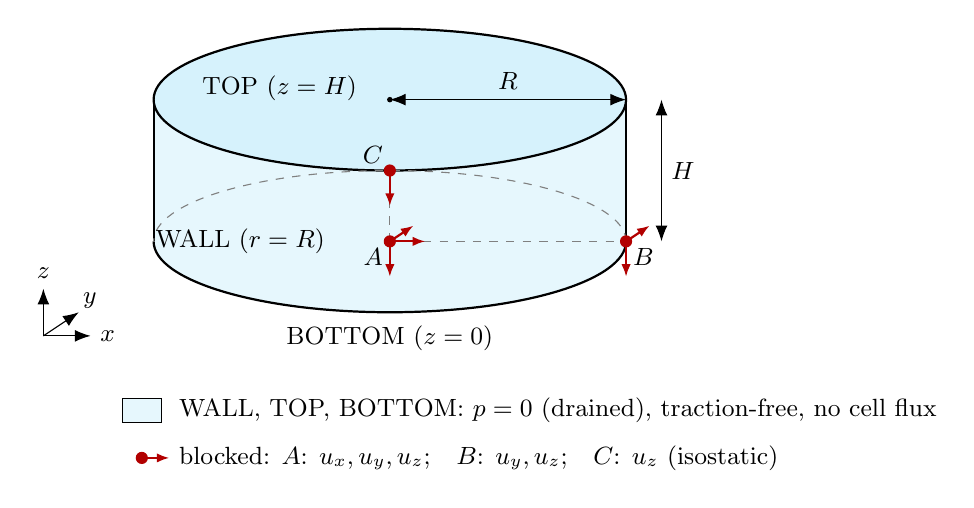
\begin{tikzpicture}[font=\small]
	% cylinder of radius R (rx = 3, ry = 0.9) and height H (1.8), oblique view from above
	\def\rx{3}\def\ry{0.9}\def\h{1.8}
	% lateral surface and top face, drained
	\fill[drained] (-\rx,0) -- (-\rx,\h) arc[start angle=180,end angle=360,x radius=\rx,y radius=\ry] -- (\rx,0)
		arc[start angle=0,end angle=-180,x radius=\rx,y radius=\ry] -- cycle;
	\fill[cyan!16] (0,\h) ellipse[x radius=\rx,y radius=\ry];
	% edges
	\draw[edge] (0,\h) ellipse[x radius=\rx,y radius=\ry];
	\draw[edge] (-\rx,0) -- (-\rx,\h) (\rx,0) -- (\rx,\h);
	\draw[edge] (\rx,0) arc[start angle=0,end angle=-180,x radius=\rx,y radius=\ry];
	\draw[hidden] (\rx,0) arc[start angle=0,end angle=180,x radius=\rx,y radius=\ry];
	% face labels
	\node at (-1.4,\h+0.15) {TOP $(z = H)$};
	\node at (-1.9,0.0) {WALL $(r = R)$};
	\node[below] at (0,-\ry-0.05) {BOTTOM $(z = 0)$};
	% dimensions
	\draw[{Latex[length=2mm]}-{Latex[length=2mm]},thin] (0,\h) -- node[above] {$R$} (\rx,\h);
	\fill (0,\h) circle (1pt);
	\draw[{Latex[length=2mm]}-{Latex[length=2mm]},thin] (\rx+0.45,0) -- node[right] {$H$} (\rx+0.45,\h);
	% support points on the bottom face (z = 0): A centre, B at (R,0,0), C at (0,R,0)
	\coordinate (A) at (0,0); \coordinate (B) at (\rx,0); \coordinate (C) at (0,\ry);
	\draw[hidden] (A) -- (B) (A) -- (C);
	\fill[support] (A) circle (2.2pt) node[below left=-1pt] {$A$};
	\fill[support] (B) circle (2.2pt) node[below right=-1pt] {$B$};
	\fill[support] (C) circle (2.2pt) node[above left=-1pt] {$C$};
	% blocked components (short arrows)
	\draw[block] (A) -- ++(0,-0.45); \draw[block] (A) -- ++(0.45,0); \draw[block] (A) -- ++(0.3,0.2);
	\draw[block] (B) -- ++(0,-0.45); \draw[block] (B) -- ++(0.3,0.2);
	\draw[block] (C) -- ++(0,-0.45);
	% axes
	\begin{scope}[shift={(-4.4,-1.2)}]
		\draw[ax] (0,0) -- (0.6,0) node[right] {$x$};
		\draw[ax] (0,0) -- (0.45,0.3) node[above right=-2pt] {$y$};
		\draw[ax] (0,0) -- (0,0.6) node[above] {$z$};
	\end{scope}
	% legend
	\begin{scope}[shift={(-3.4,-2.15)}]
		\fill[drained] (0,-0.15) rectangle (0.5,0.15); \draw (0,-0.15) rectangle (0.5,0.15);
		\node[right] at (0.6,0) {WALL, TOP, BOTTOM: $p = 0$ (drained), traction-free, no cell flux};
		\fill[support] (0.25,-0.6) circle (2.2pt); \draw[block] (0.25,-0.6) -- ++(0.35,0);
		\node[right] at (0.6,-0.6) {blocked: $A$: $u_x, u_y, u_z$;\quad $B$: $u_y, u_z$;\quad $C$: $u_z$ (isostatic)};
	\end{scope}
\end{tikzpicture}
\end{document}
